\chapter{Grundlagen}\label{kap:grundlagen}

%########################################################################################
%##########################  CHAPER 1: GRUNDLAGEN  ######################################
%########################################################################################


Computer könne in kürzester Zeit die komplexesten Berechnungen durchführen, wenn es jedoch um eine für den Menschen so 
simple Aufgabe wie das erkennen und zuordnen eines Gegenstandes auf einem Bild geht, ist diese Aufgabe praktisch 
unmöglich für einen Computer mit herkömmlicher programmierung. Da jedoch sowohl die Entwicklung von Deep Learing 
Algorithmen als auch die Rechenleistung in den letzen Jahren rasante Fortschritte gemacht haben, ist die bis vor kurzem 
noch unmöglich geglaubte Aufgabe zum alltäglichen ... im Bereich des Maschinellen Sehens geworden.\\

Um Objekte auf Bildern erkennen und lokalisieren zu können werden Künstliche Neuronale Netze zusammen mit 
Techniken der Bildverarbeitung angewandt.\\


Da Neuronale Netze oder Konkret hier Deep Learining eine Unterart des machinellen Lernens ist wird im ersten Teil der 
Einleiten kurz die wichtigsten Grundlagen des Machine Learnings eingegangen.
Anschließend wird die allgemeine Funktionsweise Künstlicher Neuronaler Netze beschrieben, welche als Grundlage zum Verst
ändnis von Convolutional Neural Networks, welche in der Bilderkennung angewand werden, dienen.  


%noch eine section zu Hardware allg (cpu, gpu, tpu), Neural Compute Stick und AI on the egde


%########################################################################################
%##########################  SECTION: MACHINE LEARNIN  ##################################
%########################################################################################

\section{Machine Learning}\label{sec:ml}


Machine Learining ist ein Teilgebiet der Computer Wissenschaften, das sich mit selbstlernenden
Algorithmen befasst. Dabei sollen Programme komplexe Zusammenhänge in einer menge von daten erkennen ohne 
expliziert dafür programmiert worden zu sein.
\\
Das unterscheidet das Vorgehen stark zur herkömmlichen Programmierung, bei dem der Entwickler bestimmte 
Regeln in einem Algorithmus definiert und dass Programm dann auf bestimmte Eingaben die richtigen Ausgaben liefert.
\\
Beim Machine Learning erhällt das Programm neben den Eingeben auch die zugehörigen Ausgaben und soll daraus dann die 
Regeln ableiten.


\begin{figure}[htb]
    \centering
    \begin{minipage}[b]{0.4\textwidth}
        \centering
        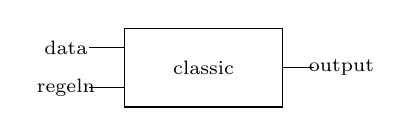
\begin{tikzpicture}[scale=0.5]
    \node at (0,1.5) {\scriptsize data};
    \node at (0,0.5) {\scriptsize regeln};
    \draw (0.6,1.5) -- (1.5,1.5);
    \draw (0.6,0.5) -- (1.5,0.5);
    \draw (1.5,0) rectangle (5.5,2);
    \node at (3.5,1) {\scriptsize classic};
    \draw (5.5, 1) -- (6.3, 1);
    \node at (7, 1) {\scriptsize output};
\end{tikzpicture}
    \end{minipage}
    \begin{minipage}[b]{0.4\textwidth}
        \centering
        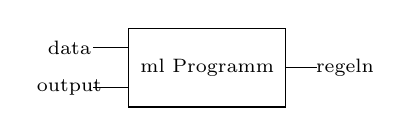
\begin{tikzpicture}[scale=0.5]
    \node at (0,1.5) {\scriptsize data};
    \node at (0,0.5) {\scriptsize output};
    \draw (0.6,1.5) -- (1.5,1.5);
    \draw (0.6,0.5) -- (1.5,0.5);
    \draw (1.5,0) rectangle (5.5,2);
    \node at (3.5,1) {\scriptsize ml Programm};
    \draw (5.5, 1) -- (6.3, 1);
    \node at (7, 1) {\scriptsize regeln};
\end{tikzpicture}
    \end{minipage}
    \caption{vgl classisches program und ml}
    \label{fig:ml_system}
\end{figure}


Dieser Prozess wird als lernen bezeichnet und ist vergleichbar mit einer mathematischen Funktion, die numerisch an die 
richtigen Ausgabewerte angenähert wird.
\\
Die Funktion bzw das Machine Lerning Model wird dabei zunächst mit zufälligen Parameter Werten initialisiert.
Anschließend werden ihr die Input Daten übergeben und das Ergebnis dieser Berechnung mit den tatsächlichen Antworten 
verglichen. Bei Abweichung werden die Parameter der Funktion in die richtige richtung angepasst. 
Dieser Prozess wird iterativ für eine vielzahl an Input Daten durchgeführt, sodass ein Model geschaffen wird, 
welches möglichst genaue vorhersagen/Schätzungen für neue Inputs abgiebt kann.
\\

Dieses Vorgehen bezeichnet man auch als \textit{Supervised Learining}. Daneben gibt es auch noch das \textit{Unsupervised Learining} 
Dabei erhält das Model neben den Input Daten keine Labels. Ziel ist es in den Daten Muster erkennen und zu gruppieren, was dem Labeln
entspricht.
\\
Zu den Haupaugaben beim Machine Learning gehören das Sammeln und aufbereiten von Daten sowie das auswählen des geeignetesten 
Models für die jeweilige Problemstellung.\\


Die Anwendugen in denen Machine Learning Algorithmen zu finden sind, sind breit gefächert.
Websiten wie Facebook, Amazon generieren (Kauf-)Vorschläge Bild und Spracherkennung, Industrie, Robotik, Selbstfahrende Autos.
Auch die Erzeugung von Bild und Ton mittels generativer Netze hat eine starke entwicklung erlebt.\\



%##########################  SUBSECTION: TRAINING  ##################################
\subsection{Training}

Ein Beispeil für einen Machine Learning Algorithmus ist die Lineare Regression. Dise soll wie in \cite{goodfellowDeepLearning2016a} 
beschrieben für einen Eingabevektor $x$ einen skalaren Ausgabewer y liefern, indem x mit einem Vektor aus parametern auch 
\textit{weights} genannt multipliziert wird.
\begin{equation}
    y = w^{T}x
    \label{eq:lin_reg}
\end{equation}


Mit hilfe einer Fehlerfunktion wird nun der Abstand der Schätung mit dem tatsächlichen Wert berechnet.
\begin{equation}
    E = \sum (y - \hat y)^{2}
    \label{eq:mse}
\end{equation}
mit $\hat y$ für den tatseächlichen Wert.\\ 
um den fehler zu minimieren müssen nun die parameter in w angepasst werden.\\
Da die fehlerfunktion quadratisch ist und von den parametern w abhängt kann durch bilden des gradienten der fehlerfunktion
für alle w bestimmt werden wie dieser angepasst werden muss:
\begin{equation}
    w  \leftarrow w - \eta \frac{\partial E}{\partial w}
    \label{eq:gradient}
\end{equation}
mit:
\begin{equation}
    \frac{\partial E}{\partial w} =  2 \sum (w^{T}x - \hat y)x
    \label{eq:gradient}
\end{equation}


Die Schritte (\ref{eq:lin_reg}), (\ref{eq:mse}) und (\ref{eq:gradient}) werden dann sooft durchgeführt, bis der Fehler 
genügend minimiert wurde.\\
Dabei können entweder alle Input Daten auf einmal verwendet werden \textit{Batch gradient Descent}, nur ein Teil \textit{Mini Batch} oder
nur ein zufallig ausgewähltes \textit{Stochastic Gradient Descent}.



Hierbei gilt es $\eta$ nicht zu groß zu wählen, um das globale Minimum der Fehlerfunktion nicht zu verpassen 
und auch nicht zu klein da das training sonst zu lange dauern würde. 

Neben der Linearen Regression werden häufig auch Modelle benötigt, deren Ausgabe eine kategorsche entscheidung trifft. 
Beispeile hierfür sind Logistische Regression, oder Suppor Vector Machine.



%##########################  SUBSECTION: VALIDIERUNG ################################
\subsection{Validierung und Overfitting}

Um zu verhindern, dass ein Model die Trainings Daten nur 'auswendig' lernt, anstatt zu generalisieren, wird während des Trainings eine 
Validierung durchgeführt. Dafür wird das Datenset in einen Trainings und in einen Test Datensatz aufgeteilt, wobei nur der Trainings
Datensatz für die Berechnung der Anpassung der Parameter Werte verwendet wird. Mit dem Test Datensatz kann dann überprüft
werden wie gut das Model die Daten generalisiert. Geht der Fehler der Trainings Daten gegen 0 wohin gegen der Test daten Fehler relativ
groß bleibt siehe %\ref{fig:overfit_loss}
spricht man von Overfitting. Dies tritt z.B. auf wenn man zu wenige Trainingsdaten hat oder das Model zu viele 
variable Parameter.

Beim Underfitting hat das Model nicht genügend Parameter um die Daten anzugleichen. Beispiel % \ref{abb 3 bilder}
mit einer Geraden and Datenpunkte mit Verlauf höhren Grad anpassen.

Um Overfitting zu vermeiden können entweder mehr Trainingsdaten, oder Regularisierung verwendet werden.
Regularisierung ist eine Technitk, die dafür sorgt, dass das model sich nicht nur den daten anpasst, sondern auch versucht die 
parameter/gewichte dabei möglichst klein zu halten. Dafür wird der zu minimierenden Loss Function als weiterer 
Therm eine aufsummierung aller quadrieten Gewichte hinzugefügt. \cite{geronHandsonMachineLearning2017}

\begin{equation}
    J(w) = E + \lambda \sum w^{2}
\end{equation}




%########################################################################################
%##########################  SECTION: NEURAL NETWORKS  ##################################
%########################################################################################
\section{Künstliche Neuronale Netze} \label{sec:nn}


Künstliche Neuronale Netze sind eine Form des Machine Learning, bei der das Modell, inspiriert vom menschlichen
Gehirn, aus mehreren miteinander verbundenen Einheiten zusammengesetzt ist. Die Einheiten auch Neuronen 
genannt sind dabei in Schichten angeordnet. Die Eingabeschicht erhällt die zu berechnenden Inputs. Ihr folgen
eine oder mehrere versteckte Schichten, welche die Inputs bis zu letzten Schicht, welche den gewünschten Output
liefern soll, duchreichen.
\\
Die berechnungen an einem einzelnen Neuron sind dabei nicht sehr komplex und gleichen der berechnung der 
in \ref{sec:ml} beschrieben Logistischen regresseion.
Wie in BILD dargestellt, werden die mit $w$ gewichteten Inputs $x$ aufsummiert und an die Aktivierungsfunktion
$g(z)$ übergeben.
\begin{figure}[htb]
    \centering
    \begin{tikzpicture}[
    % define styles    
    init/.style={ 
         draw, 
         circle, 
         inner sep=2pt,
         font=\Huge,
         join = by -latex
    },
    squa_draw/.style={ 
        draw,
        font=\Large,
        join = by -latex
    },
    squa/.style={ 
        font=\Large,
        join = by -latex
    }
]
% Top chain x1 to w1
\begin{scope}[start chain=1]
    \node[on chain=1] at (0,1.5cm)  (x1) {$x_1$};
    \node[on chain=1,join=by o-latex] (w1) {$w_1$};
\end{scope}
% Middle chain x2 to output
\begin{scope}[start chain=2]
    \node[on chain=2] (x2) {$x_2$};
    \node[on chain=2,join=by o-latex] {$w_2$};
    \node[on chain=2,init] (sigma) {$\displaystyle\Sigma$};
    \node[on chain=2,squa_draw,label=below:{\parbox{2cm}{\centering Aktivierungs-funktion}}]   {$g(z)$};
    \node[on chain=2,squa,label=below:Output,join=by -latex] {$y_{out}$};
\end{scope}
% Bottom chain x3 to w3
\begin{scope}[start chain=3]
    \node[on chain=3,label=below:Inputs] at (0,-1.5cm) 
    (x3) {$x_3$};
    \node[on chain=3,label=below:Gewichte,join=by o-latex]
    (w3) {$w_3$};
\end{scope}
% Bias
\node[label=above:\parbox{2cm}{\centering Bias \\ $b$}] at (sigma|-w1) (b) {};
% Arrows joining w1, w3 and b to sigma
\draw[-latex] (w1) -- (sigma);
\draw[-latex] (w3) -- (sigma);
\draw[o-latex] (b) -- (sigma);

\end{tikzpicture}

% von https://medium.com/momenton/typesetting-neural-network-diagrams-with-tex-4920b6b9fc19
    \caption{Einzelnes Perzeptron}
    \label{fig:neuron}
\end{figure}

\textbf{hier bild von neuron}
\\
Wie in bei der Logistische Regression \ref{sec:ml} wird zunächst der Fehler mittels Loss Funktion berchnet und 
anschließend nach dem Gradienten verfahren die Anpassungen für die Parameter/Gewichte $w$ bestimmt.
\\


% hier bild von einzelnen neuron + formel

% Sie sollen damit die Funktions- und Lernweise des Menschlichen Gehirns nachahmen.


% verbindungen sind unterschiedlich stark gewichtet, 
% Inspiriet vom Menschlichen Gehin stellen sie ein vielzahl miteinander verbundener 
% künstlicher Neuronen dar, die Informationen übertragen können. Ein solches Netz besteht aus einer Eingabeschicht, 
% einer oder mehreren Hidden Schichten und einer Ausgabeschicht.
% Durch unterschiedlich starke gewichtung der Verbindungen soll das Netz für bestimmte Inputs 
% (auf die es trainiert wurde) die gewünscshten Outputs liefern.
% \\
% Jedes der Neuronen auch Perzeptron genannt erhällt dabei die Outputs der voerigen schicht, multipliziert mit den
% jeweiligen Gewichten, summiert diese auf und übergibt sie einer Aktivierungsfunktion.
% \\
% Ein einzelnes Neuron berechnet sich dabei ähnlich wie die in \ref{sec:ml} beschrieben Lineare Regression, mit Aktivierungs
% Function.


%##########################  SUBSECTION: MLP  ##################################
\subsection{Mehrschichtiges Netz}

Um komplexere Zusammenhänge in Daten zu lernen ist eine verschaltung der Neuronen in Netzwerkartiger Struktur ref BILD
notwendig. Für die Anzahl der Hidden Schichten und Neuronen in diesen gibt es keine definierten Vorgeaben. Lediglich 
die Zahl der In- und Output Neuronen ist vorgegeben.

\begin{figure}
    \centering
    \input{Bilder/neuralnetwork.tex}
    \caption{Neural Network Struktur}
    \label{fig:nn}
\end{figure}

Die berechnungen von einer Schicht zu nächsten entspricht der Matrixmultiplikatin der Werte an der aktuellen Schcht 
mit den Gewichten der Verbindungen $w$ zur nächsten Schicht.



\begin{equation}
    \label{mat:feedforward}
    \begin{pmatrix}
        x_{0} & x_{1} & x_{2}
    \end{pmatrix}
    \cdot
    \begin{pmatrix}
        w_{0,1} & x_{0,2}\\
        w_{1,1} & x_{1,2}\\
        w_{2,1} & x_{2,2}\\
    \end{pmatrix}
    =
    \begin{pmatrix}
        y_{1}\\
        y_{2}
    \end{pmatrix}
\end{equation}\\

oder:

\begin{equation}
    \label{eq:nn}
    y = \delta(w_{0} + w^{T}x)
\end{equation}

wobei die Aktivierungsfunktion $\delta(z)$ dazu dient den Wert auf einen bestimmten Bereich zu skalieren.\\

\subsection{Aktivierungs- und Lossfunktionen}
Gängige Aktivierungsfunktion sind:\\
\textit{Sigmoid}: erzeugt nicht-linearität und skaliert zw 0 und 1.
\begin{equation}
    \label{eq:sigm}
    \delta(z) = \frac{1}{1 + e^{-z}}
\end{equation}


\textit{ReLu}: setz die negativen Werte zu null (warum von vorteil).
\begin{equation}
    \label{eq:relu}
    \delta(z) = max(0,z)
\end{equation}


\textit{Softmax}: oft in der letzten Schicht verwendet (bei kategrischer Classification), welche eine 
Wahrscheinlichkeitsverteilung über allen Output Neuronen, die sich zu 1 aufsummeiren lässt, bildet.
\begin{equation}
    \label{eq:softmax}
    \delta(z) = \frac{e^{z}}{\sum e^{x}}
\end{equation}

Die Ergebnisse der Aktivierungsfunktionen einer Schich dienen dann als Inputvektor für die nächste Schicht.
An der Output Schicht wird nun der Fehler mittels Loss Funktion berechnet. Neben der in \ref{sec:ml} für 
Lineare Regression verwendeten \textit{Mean Squre Error} funktion wird für Klassifikationsprobleme häufig 
die \textit{Cross Enropy Fehlerfunktion} verwendet.

\begin{equation}
    \label{eq:crossentropy}
    E = -\sum\hat{y}log(y)
\end{equation}

Mit $\hat{y}$ für den tatsächlichen Wert (1 oder 0) und $y$ als den geschätzen Wert (zwischen 0 und 1).
Durch den Logarithmus wird der Loss besonders gross, für Werte die fälschlicher Weise 0 oder 
richtung 0 geschätzt wurden.


%##########################  SUBSECTION: BACKPROPAGATION  ###############################
\subsection{Backpropagation}
Um nach dem Gradienten Verfahren die Werte für die Anpassungen aller Gewichte $w$ zu bestimmen, müssen die Ableitungen
über die Kettenregel bestimmt werden. Dabei werden zunächst die Partiellen Ableitungen nach den Gewichtien der
letzen Schicht bestimmt. Mit diesen die für die der voletzen, usw bis zur vordersten schicht.

\begin{equation}
    \frac{\partial E}{\partial w} = \frac{\partial E}{\partial y}\frac{\partial y}{\partial z}\frac{\partial z}{\partial w}
\end{equation}

Um damit die Gewichte anzupassen:

\begin{equation}
    w  \leftarrow w - \eta \frac{\partial E}{\partial w}
    \label{eq:gradient}
\end{equation}

Wie bei der in \ref{sec:ml} beschriebenen Linearen Regression, werden nun auch beim Training des Neuronalen 
Netzes die Schritte
\begin{enumerate}
    \item \textit{Forward Propagation} für eine Anzahl N an Inputs
    \item Berechnung der \textit{Loss Funktion}
    \item \textit{Backpropagation} und Anpassung der Gewichte
\end{enumerate}
sooft wiederholt, bis der Fehler ausreichend minimiert wurde.
% überlegun: trainingsprozess aus ml teil rausnehmen, da sonst viel doppelt





%##########################  SUBSECTION: FRAMEWORKS  ####################################
\subsection{Machine Learning Frameworks}


%########################################################################################
%##########################  SECTION: DEEP LEARNIN UNG COMPUTER VISION  #################
%########################################################################################
\section{Deep Learning und Computer Vision}\label{sec:deepl_cv}


Neben den in \ref{sec:nn} beschrieben \textit{Feed Forwar Netzen} gibt es eine vielzahl and erweiterungen, die jedoch alle das 
Grundprinzip verwenden.\\

deep wegen mehr als 1 hidden schicht\\

Arten von NNs:
\begin{itemize}
    \item CNN: für bilder, durch faltung erkennt features und ist translatorisch invariant: \textbf{Image Classification}
    \item Recurrecnt Neural Networks/LSTM: durch feedback in network: für Audio und zeitl. anwendungen 
    \item Autoencoder: 
    \item \dots
\end{itemize}

hier geht es um in bla beschriebene cnns\\


%##########################  SUBSECTION:CNNs  ################################
\subsection{Convolutional Neural Networks}


Auch hier wieder biologische inspiration: Auge Rezeptives Feld

math faltung\\


Conv layer:\\
Faltung an cnn erklärt: input image als (h,w,c) tensor wird mit filter/kernel gefaltet. daraus erhält man feature map
zusammen mit pool layer:\\
pool layer erklärt\\

ergibt grundstruktur von cnn\\

weitere layer wie dropout\\

%##########################  SUBSECTION: TANSFER LEARINING  ################################
\subsection{Transfer Learining}

erklären, dass features von einfach bis immer komplexer werdende muster enthalten, die im bild zu finden sind.
\\
filter können zufällig initialisiert und gelernt werden, oder von vortrainierten netzen wieder verwendet
werden. (transfer learining oder fine tuning) da die deatures (besonders in den vorderen layern) immer ähnlich sind und das
neu lernen zeitaufwändig und oft sogar ungenauer ist.
\\
je nach ähnlichkeit des eig datensetz zu dem auf das netz urspr trainiert wurde:\\
scratch, fine tuning, feature extractor



%##########################  SUBSECTION: COMPETITIONS  ################################
\subsection{Competitions mit Imagenet und co + cnn winner}\label{subsec:comp}

zuerst competition erklären \\
dann chronologische gewinner netzt + besonderheit\\




%##########################  SUBSECTION: OBJEKT ERKENNUNG  ################################
\subsection{Objekt erkennung}\label{sec:objdet}


Unterschied deutlich machen: klassifikator kann nur ges bild auswertuen und wahscheinlichk angeben welche 
klasse darauf. keine lokalisierng und keine mult obj\\

3 Arten der Bilderkennung: Klassifizierung, Objekt Erkennung (für mult + box), Segmentation (jeden pixel)

dafür obj erkennung notw:\\

Single Shot Detectoren
\\

Two Stage Detectoren


%########################################################################################
%##########################  SECTION: HARDWARE  #################
%########################################################################################
\section{Hardware}\label{sec:hardware}
%noch eine section zu Hardware allg (cpu, gpu, tpu), Neural Compute Stick und AI on the egde


allg zu hardware für deeplearning. Das besser auf gpu als cpu. weitere: tpu, fpga, vpu, wie zb ncs2.

\subsection{Neural Compute Stick 2}

technischen spezifikationen





\subsection{AI on the edge}

was bedeutet dies. cloud unabhängig und ohne groß rechner. bsp anwendungen.

